%==================================================
%      PREAMBOLO e DICHIARAZIONI INIZIALI
%==================================================
\documentclass[10pt,oneside,a4paper]{article}

\usepackage[latin1]{inputenc} 
\usepackage[italian]{babel}
\usepackage{siunitx} %Inserisce automaticamente i dati con le unit�  di misura correttamente formattate del SI (utilizzo: \SI{0.82}{m^2}, in generale \SI{misura con il punto decimale}{unit�  di misura})
\sisetup{output-decimal-marker = {.}, separate-uncertainty = true, input-uncertainty-signs = \pm, detect-weight=true, detect-family=true} %per usare SI con il punto decimale
\usepackage{listings} %Per citare codice informatico formattandolo correttamente
\usepackage{amsmath,amsthm,verbatim,amssymb,amsfonts,amscd, graphicx,mathtools}
\usepackage[makeroom]{cancel}
\newcommand{\abs}[1]{\left\lvert\,#1\,\right\rvert}
\usepackage{geometry}
\usepackage{epigraph}
\usepackage{booktabs}	%tabelle migliorate
\usepackage{tablefootnote}	%note a pi� di pagina in tabella
\usepackage{threeparttable} %tabella con note a pi� di tabella
\usepackage{caption}	%descrizione per figure
\usepackage{dblfnote}
\captionsetup{tableposition=top,figureposition=bottom,font=small} %setup descrizione
\usepackage{float}
\usepackage{esvect} %vettori
\usepackage{longtable} %tabelle lunghe
\usepackage[dvipsnames]{xcolor}
\definecolor{sepia}{HTML}{80002A}
\usepackage[colorlinks=true, citecolor=black, linkcolor=sepia, urlcolor=black]{hyperref}
\usepackage{mathrsfs}
%\usepackage[utf8]{inputenc}

\usepackage{multicol}
\newenvironment{Figure}
  {\par\medskip\noindent\minipage{\linewidth}}
  {\endminipage\par\medskip}


\newcommand{\var}{\operatorname{var}}
\newcommand{\cov}{\operatorname{cov}}


\usepackage{listings} %Per inserire codice
\lstnewenvironment{codice_c}[1][]
{\lstset{basicstyle=\small\ttfamily, columns=fullflexible,
keywordstyle=\color{red}\bfseries, commentstyle=\color{blue},
language=C, basicstyle=\small,
numbers=left, numberstyle=\tiny,
stepnumber=2, numbersep=5pt, frame=shadowbox,  showstringspaces=false, #1}}{}

\setcounter{section}{-1}

%==================================================
%                  PRIMA PAGINA
%==================================================

\title{\textsc{Variazione della tensione di vapore saturo dell'acqua con la temperatura}}
\author{\small{G. Galbato Muscio} \and \small{L. Gravina} \and \small{L. Graziotto}}
\date{}

\begin{document}
	\begin{figure}
		\centering
		\includegraphics[scale=0.5, trim={2.8cm 8.9cm 0 9cm}, clip]{logo.png}
	\end{figure}
	\maketitle
	\begin{center} 
		\fbox{{\fontsize{12pt}{8mm}\textsc{Gruppo B}}} \\
		\vspace{1cm}
		\begin{tabular}{ccc}
			Esperienza di laboratorio && Consegna della relazione \\
			\emph{\small{11 dicembre 2017}} &&  \emph{\small{15 gennaio 2018}}\\
		\end{tabular} 
		\vspace{0.5cm}
	\end{center}
\hrule
\vspace{0.5cm}
\begin{abstract}
Si studia la dipendenza della tensione di vapore saturo, ossia la pressione alla quale si ha ebollizione di un liquido, dalla temperatura del liquido stesso. Dall'equazione di Clausius-Clapeyron, che regola il fenomeno, si ricava sperimentalmente il calore latente di evaporazione del liquido. Il liquido utilizzato � acqua.
\end{abstract}
\newpage
\tableofcontents %Indice
\listoftables %Indice delle tabelle
\listoffigures %Indice dei grafici

\pagebreak
\begin{multicols}{2}

%==================================================
%         SCOPO E DESCRIZIONE DELL'ESPERIENZA
%==================================================
\section{Scopo e descrizione dell'esperienza}
\label{sec:descrizione}
L'ebollizione di un liquido avviene quando l'evaporazione non riguarda unicamente le molecole a contatto diretto con l'ambiente esterno, ma anche porzioni di liquido interne: tale fenomeno pu� verificarsi unicamente quando la pressione di vapore saturo, ossia quella di equilibrio tra fase gassosa del sistema e fase liquida, eguaglia la pressione applicata sul sistema termodinamico nel suo insieme. La temperatura di ebollizione di un liquido � dunque definita in relazione alla pressione $P$ applicata sul sistema, ed � quella a cui la tensione di vapore saturo uguaglia $P$.

L'esperienza si propone di studiare la dipendenza della tensione di vapore saturo dalla temperatura, portando il liquido, in questo caso acqua, ad una certa temperatura, e quindi diminuendo la pressione del sistema termodinamico chiuso in modo da portare il liquido all'ebollizione: la pressione raggiunta sar� pari alla tensione di vapore saturo.

La diminuzione di pressione nel sistema chiuso � ottenuta mediante una pompa rotativa, collegata al sistema termodinamico mediante tubi che passano attraverso una camera in vetro immersa in azoto liquido: tale componente del \emph{setup} sperimentale ha lo scopo di intrappolare, condensandolo, il vapor d'acqua in uscita dal sistema termodinamico, affinch� esso non contamini l'olio lubrificante della pompa stessa, diminuendone le prestazioni.

Si prevede un andamento crescente della tensione di vapore saturo in funzione della temperatura, ovvero che a pressioni maggiori la temperatura di ebollizione sia pi� elevata: � necessaria un'energia cinetica maggiore, dunque una temperatura maggiore, delle molecole del liquido per vincere infatti la pressione applicata sul sistema e passare dalla fase liquida a quella gassosa.

Si procede quindi a confrontare l'andamento ottenuto per via sperimentale con quello previsto per via teorica dall'equazione di Clausius-Clapeyron: eseguendo un'interpolazione tra le due curve, si ricava sperimentalmente il valore del calore latente di evaporazione dell'acqua.

Per l'analisi dati si utilizzer� un notebook in linguaggio \texttt{Python}.


%==================================================
%				APPARATO SPERIMENTALE
%==================================================		
\section{Apparato Sperimentale}
\subsection{Strumenti}
\label{subsec:strumenti}
\begin{itemize}
	\item Recipiente in pyrex in cui � inserita $n = \SI{1}{mol}$ di $H_2O$;
	\item Resistenza elettrica inserita nel recipiente di cui sopra, collegata con un generatore di tensione;
	\item Pompa rotativa che permette di variare la pressione nel recipiente di cui sopra;
	\item Camera in vetro immersa in un bagno di azoto liquido a $T = \SI{77}{K}$, collegata da una parte al recipiente di cui sopra e dall'altra alla pompa rotativa;
	\item Rubinetti tra la camera in vetro e il recipiente e tra il recipiente e l'ambiente esterno.
\end{itemize}
\subsection{Sensori}
\begin{itemize}
	\item Manometro [risoluzione: \SI{1e-4}{bar}];
	\item Termometro a mercurio [risoluzione: \SI{0.2}{\degree C}, incertezza \SI{0.03}{\degree C}].
\end{itemize}

%==================================================
%            SEQUENZA OPERAZIONI SPERIMENTALI
%==================================================
\section{Sequenza Operazioni Sperimentali} 

\paragraph{Modello fisico ideale}
La relazione che lega la tensione di vapore saturo alla temperatura di ebollizione � l'\textbf{equazione di Clausius-Clapeyron}
\large{
\begin{equation}\label{eq:clausius-clapeyron}
P =  P_0 e^{-\frac{\lambda_\text{ev} M}{R} \big(\frac{1}{T} - \frac{1}{T_0}\big) }
\end{equation}
}
\normalsize
Dove $\lambda_\text{ev}$ rappresenta il calore latente di evaporazione, $M$ � la massa molare del liquido, $R$ � la costante universale dei gas e $P_0$, $V_0$ indicano i valori di pressione e temperatura di un punto nel piano pressione-temperatura assunto come riferimento.

\paragraph{Situazione reale}
Il sistema termodinamico � costituito da una massa d'acqua allo stato liquido di \SI{18}{g}; ricordando che la massa molare � \SI{18}{g/mol}, si pu� esprimere la quantit� presente come \SI{1}{mol}. A partire dall'equazione~\ref{eq:clausius-clapeyron} ci si prefigge di ricavare sperimentalmente il valore del calore latente di evaporazione $\lambda_\text{ev}$, che si confronter� con il valore vero di \SI{539.31}{cal / g}. In questo caso, si utilizzer� il valore della costante dei gas $R = \SI{1.987}{cal / (K \cdot mol)}$

Si eseguono $10$ prese dati della tensione di vapore saturo variando la temperatura del liquido nell'intervallo $38 \div 82$ \SI{}{\degree C}; si osserva, in particolare, che una volta portato il liquido a temperatura, riscaldandolo mediante la resistenza elettrica e con il rubinetto a contatto con l'ambiente esterno aperto, quando quest'ultimo viene chiuso e la pressione viene diminuita anche la temperatura diminuisce: si ritiene che questo sia dovuto in parte alla non adiabaticit� delle pareti del recipiente, in parte alla fuga delle molecole gi� allo stato aeriforme che vengono portate al di fuori dal sistema termodinamico dall'azione della pompa rotativa, e fatte condensare nella camera immersa in azoto liquido. Si reputa pertanto che alla fine dell'esperimento la quantit� di acqua presente nel recipiente sar� sensibilmente inferiore a quella presente inizialmente.

I punti relativi alla tensione di vapore saturo ad una data temperatura vengono rappresentati in un grafico semilogaritmico: l'equazione di Clausius-Clapeyron~\ref{eq:clausius-clapeyron} viene pertanto riscritta come
\begin{equation*}
\log{\Big(\frac{P}{P_0}\Big)} = \frac{\lambda_\text{ev} M}{R} \Big(\frac{1}{T_0} - \frac{1}{T} \Big),
\end{equation*}
da cui � chiara la dipendenza del logaritmo della pressione, rapportata alla pressione di riferimento, dall'inverso della temperatura di ebollizione.

Ancora, indicando con $m$ il coefficiente angolare della retta che interpola i punti sperimentali nel grafico semilogaritmico, si ha 
\begin{equation}\label{eq:calore_latente} 
\lambda_\text{ev} = - \frac{m R}{M},
\end{equation}
ove l'unit� di misura del coefficiente $m$ � [\SI{}{K}] e quella del calore latente � [\SI{}{cal / g}].


\paragraph{Procedura e presa dati}
Una volta organizzato l'apparato sperimentale � necessario tarare il manometro avendo cura di lasciare aperta la valvola che separa l'ambiente esterno dall'ampolla contenente il liquido, in modo da tarare a \SI{0}{bar} la pressione atmosferica: � sufficiente eseguire questa operazione solamente all'inizio della presa dati. Si procede quindi come segue
\begin{enumerate}
	\item A pressione atmosferica (quindi con la valvola $\mathrm{R}_2$\footnote{Con $\mathrm{R}_2$ ci si riferisce alla valvola che separa l'ampolla dall'ambiente.} aperta) si porta l'acqua ad una temperatura $\tilde{T}$.
	\item Con la pompa del vuoto accesa, si chiude la valvola $\mathrm{R}_2$ e si apre $\mathrm{R}_1$\footnote{Con $\mathrm{R}_1$ ci si riferisce alla valvola che separa l'ampolla dalla pompa del vuoto.} in modo da abbassare la pressione all'interno dell'ampolla.
	\item Si abbassa la pressione fino a che si distinguono i primi segni evidenti dell'ebollizione dell'acqua (formazione di bolle che si muovono dal fondo alla superficie, increspatura e movimento della superficie dell'acqua).
	\item Si prende la coppia di misure di pressione-temperatura $(\mathrm{P}, \mathrm{T})$ con $\mathrm{T} < \bar{T}$ perch�, come accennato in precedenza, nel procedimento l'acqua avr� scambiato calore con l'ambiente circostante.
	\item Si chiude $\mathrm{R}_1$ e si riporta l'ampolla a pressione atmosferica aprendo $\mathrm{R}_2$.
\end{enumerate}

I dati raccolti sono riportati nella tabella \ref{tab:misure}, nel grafico \ref{fig:grafico} sono invece riportati i valori del logaritmo $\log (P/P_0)$ al variare della quantit� $1/T$, insieme al fit lineare dei dati.

\begin{table*}
\begin{center}
\begin{tabular}{cc}
	$P$ & $T$ \\
	$[\SI{}{kPa}]$ & $[\SI{}{K}]$ \\
	$\pm 0.01$ & $0.03$ \\
	\toprule
	7.79 & 312.05 \\
	10.89 & 318.35 \\
	12.50 & 321.85 \\
	17.77 & 329.55 \\
	22.13 & 334.35 \\
	27.90 & 340.15 \\
	30.41 & 341.55 \\
	36.04 & 345.75 \\
	43.17 & 350.45 \\
	50.02 & 354.55 \\
	
\end{tabular}	
\captionof{table}{Valori di temperatura e pressione ai quali si � osservata l'ebollizione.}
\label{tab:misure}
\end{center}
\end{table*}

%INSERIRE IL GRAFICO DI LOG(P/P0) SU 1/T (dall'iPad ho problemi con le figure)
\begin{Figure}
\centering
\hspace*{-2cm} 
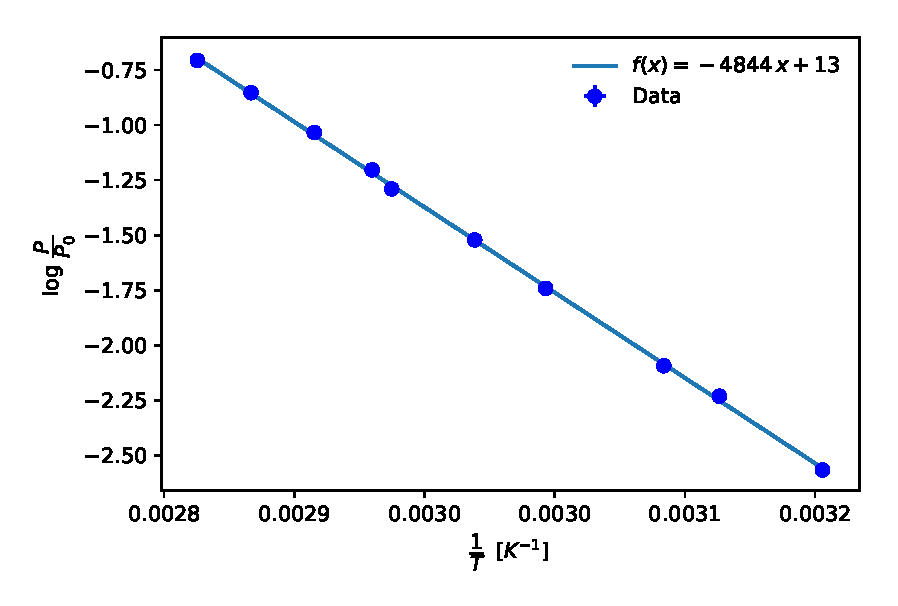
\includegraphics[width=9cm, height=6cm]{fit.eps}
\captionof{figure}{Andamento della pressione in funzione del tempo, $\Delta V = \SI{10}{mL}$}
\label{fig:Pvst-compression}
\end{Figure}



\paragraph{Analisi dati}
Un preliminare test del $\chi^2$ sul fit produce un valore incompatibile con il modello lineare previsto: essendo l'andamento delle quantit� evidentemente lineare, un tale risultato � indice di una sottostima delle incertezze sull'asse delle ordinate (che a priori � la propagazione dell'errore strumentale del manometro sulla quantit� $\log (P/P_0)$), quindi si inferiscono gli errori sui logaritmi a partire dal fit e si ristimano le incertezze sui parametri del fit stesso.
Si calcolano infine i parametri del fit lineare, pari rispettivamente a
\begin{equation*}
	m = \SI{-4844 \pm 43}{T^{-1}}, \quad q = \SI{12.97 \pm 0.13}{}.
\end{equation*}

Utilizzando (\ref{eq:calore_latente}) si calcola il calore latente di ebollizione dell'acqua, pari a
\begin{equation*}
	\boxed{\lambda_{\mathrm{ev}} = \SI{534.7 \pm 4.8}{cal/g}	}
\end{equation*}
compatibile con il \emph{valore vero} pari a $\lambda_{\mathrm{ev}} = \SI{539.31}{cal/g}$ in una $\sigma$.

L'incertezza su tale parametro � stata ottenuta propagando l'incertezza sul coefficiente angolare su (\ref{eq:calore_latente}), con la formula
\begin{equation*}
	\sigma_{\lambda}^2 = \Big(-\frac{R}{M}\Big)^2 \sigma_\mathrm{m}^2	
\end{equation*}
dove le quantit� $\mathrm{R} = \SI{1.987}{cal \cdot K^{-1} \cdot mol^{-1}}$ e $ \mathrm{M} = \SI{18}{g}$ si sono prese senza incertezze.

%==================================================
%				CONSIDERAZIONI FINALI
%==================================================
\section{Considerazioni finali}



\end{multicols}
\end{document}